% 第三章 系统需求分析

\chapter{系统需求分析}
\label{chap:requirements-analysis}

系统需求分析是系统设计与实现之前的重要环节。对于在线视频分享平台而言，需求分析不能只停留在“能够播放视频”这一层面，还需要从用户角色、业务流程、功能边界、内容审核、性能要求和系统可行性等方面进行分析。本章主要围绕系统总体需求、用户端需求、创作中心需求、管理端与 AI 审核需求、非功能需求以及可行性分析展开。

\section{系统总体需求分析}
\label{sec:overall-requirements}

\subsection{需求分析目标}
\label{subsec:req-analysis-goal}

本课题旨在设计并实现一个基于微服务架构的在线视频分享平台。系统需要围绕视频内容的生产、处理、审核、发布和消费形成完整闭环。普通用户可以浏览、搜索和播放视频，并参与评论、弹幕、点赞、收藏、投币等互动；内容创作者可以上传视频、编辑投稿和管理个人作品；管理员可以在后台进行分类维护、视频审核和内容治理；AI 审核服务则负责对上传视频进行自动化风险识别，为人工审核提供辅助依据。图~\ref{fig:system-functional-structure} 
展示了系统的功能结构图。

\begin{figure}[htbp]
    \centering
    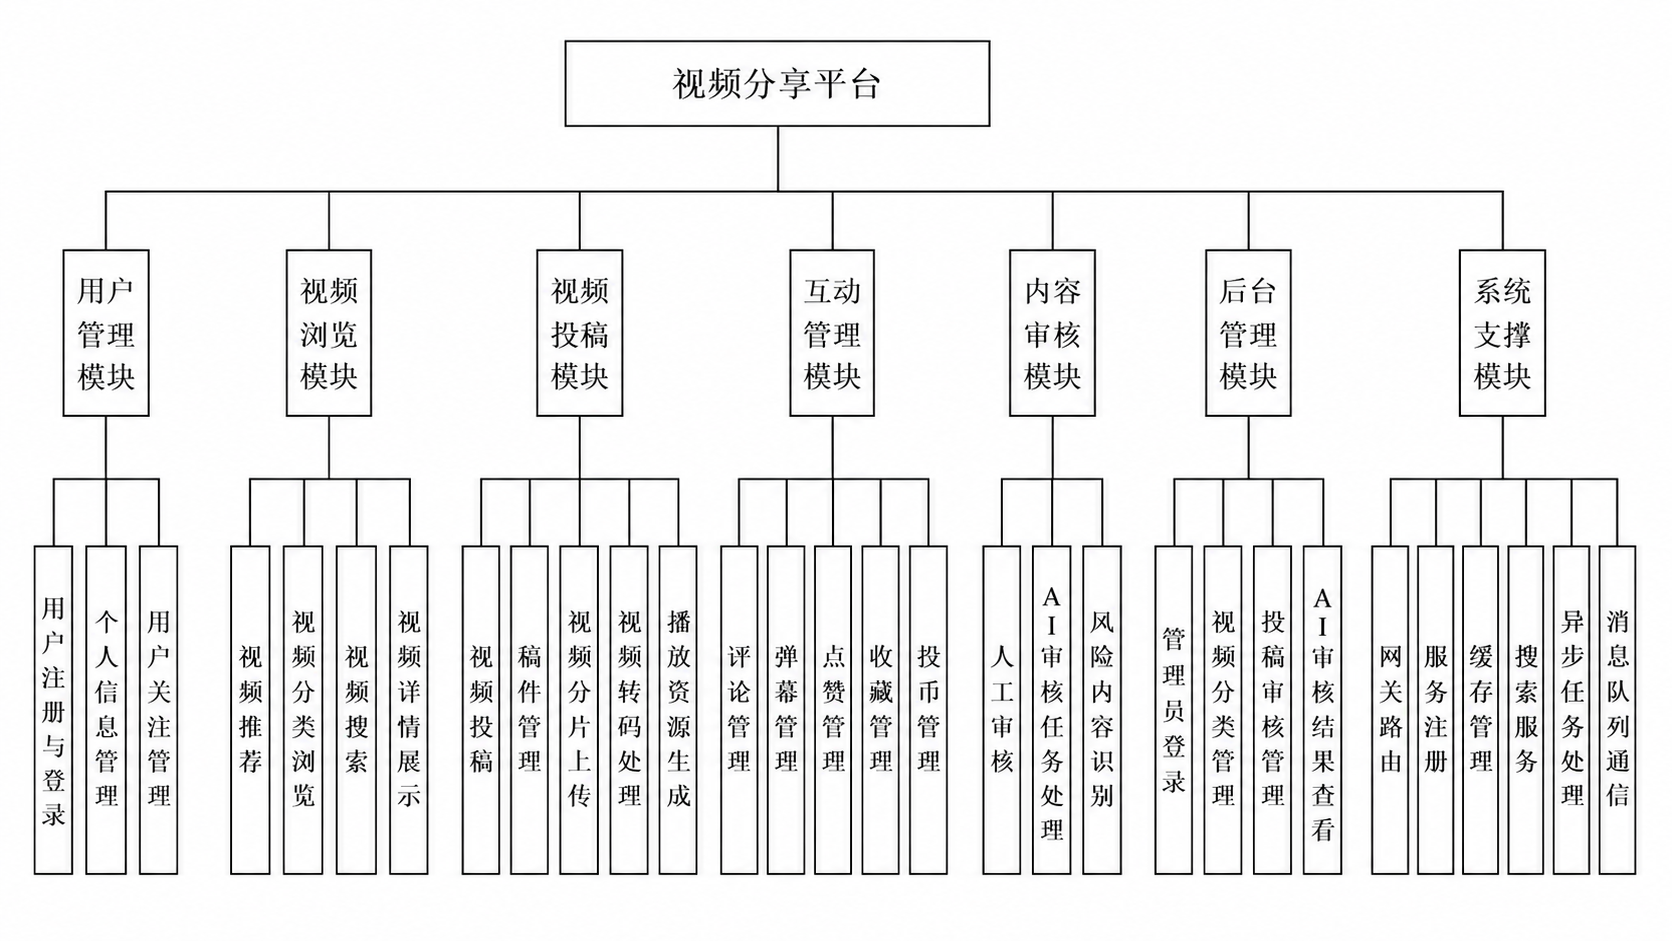
\includegraphics[width=0.95\textwidth]{images/system_functional_structure.png}
    \caption{系统功能结构图}
    \label{fig:system-functional-structure}
\end{figure}

\subsection{系统参与角色划分}
\label{subsec:system-actors}

为了明确系统中不同用户和外部服务的权限边界，本系统根据业务参与方式和功能访问范围，将参与角色划分为未登录访问者、注册用户、内容创作者、系统管理员和 AI 审核服务五类。系统用例图如图~\ref{fig:system-use-case} 所示。

\begin{figure}[htbp]
    \centering
    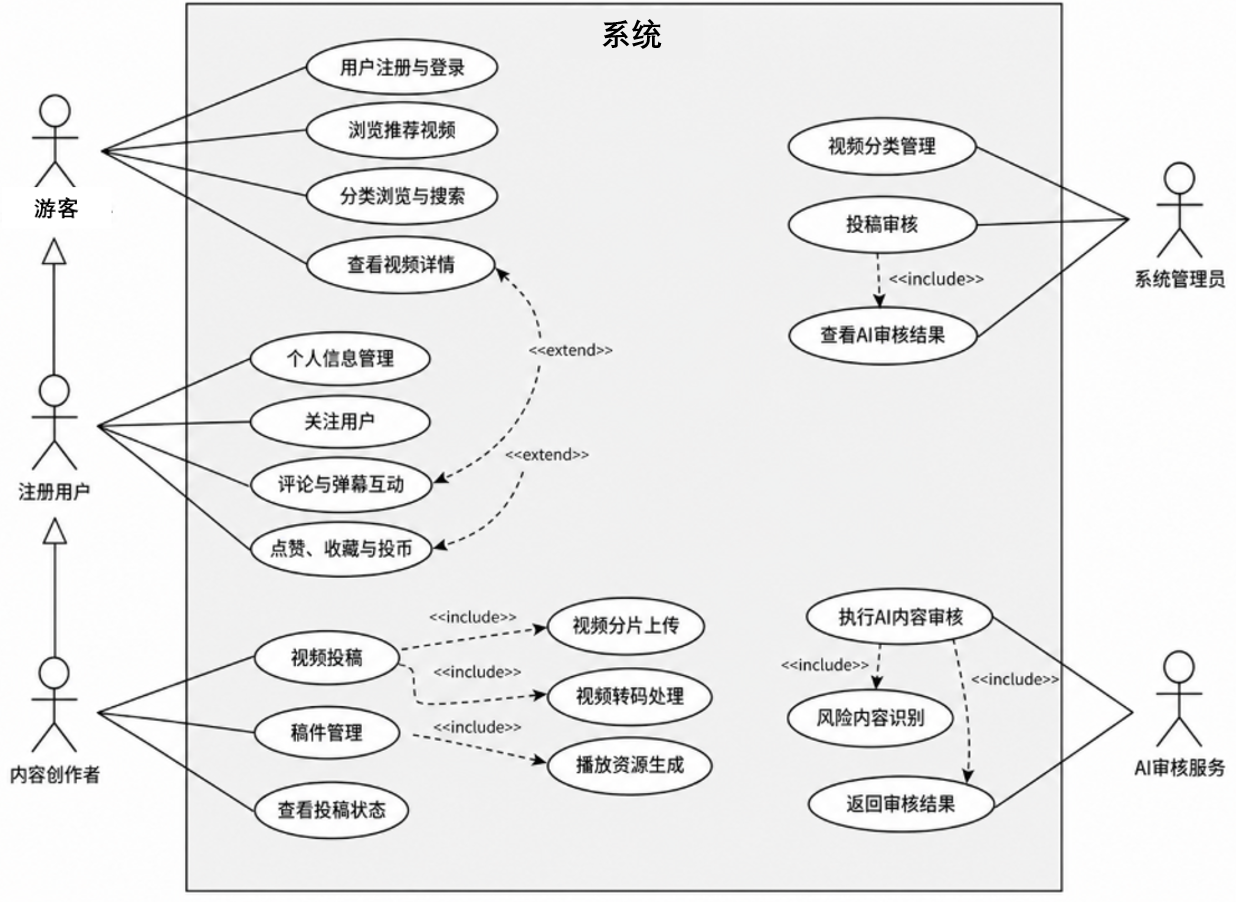
\includegraphics[width=0.95\textwidth]{images/system_use_case.png}
    \caption{视频分享平台系统用例图}
    \label{fig:system-use-case}
\end{figure}

游客是系统中的基础访问角色，主要使用平台的公开浏览功能。该类用户可以进行用户注册与登录、浏览推荐视频、分类浏览与搜索以及查看视频详情等操作，但不能进行评论、弹幕、点赞、收藏、投币和投稿等需要身份认证的行为。

注册用户是在游客基础上完成账号登录后的用户角色，因此继承了基础浏览能力，并进一步具备个人信息管理、关注用户、评论与弹幕互动、点赞、收藏和投币等功能。注册用户是平台互动行为的主要参与者，其操作能够增强视频内容的传播和用户之间的交互。

内容创作者是注册用户的扩展角色，主要负责视频内容的提交与管理。该类角色除具备注册用户的基本功能外，还可以进行视频投稿、稿件管理和查看投稿状态等操作。在视频投稿过程中，系统会包含视频分片上传、视频转码处理和播放资源生成等子功能，以保证视频资源能够被正常存储、处理和播放。

系统管理员主要负责后台管理与内容监管工作。管理员登录后台后，可以进行视频分类管理、投稿审核以及 AI 审核结果查看等操作。其中，投稿审核过程会包含对 AI 审核结果的查看，以便管理员结合自动审核结果对投稿内容进行人工复核，从而提高内容审核的准确性和规范性。

AI 审核服务是系统中的外部自动化审核参与者，主要用于辅助完成视频内容审核。该服务接收后端系统提交的审核任务后，执行 AI 内容审核，并在审核过程中完成风险内容识别，最终将审核结果返回给后端系统，为管理员的人工审核提供参考依据。

\subsection{系统总体业务流程}

在线视频分享平台的核心流程可以概括为“内容生产、内容处理、内容审核、内容发布、内容消费”。视频在公开展示前需要完成上传、转码和审核，避免未经处理或未经审核的内容直接进入前台。

视频平台业务并不是简单的同步请求流程，而是由上传、转码、审核、发布和消费多个阶段组成。其中，上传阶段主要由内容创作者完成，用于提交视频文件、标题、简介、分类、封面等投稿信息；转码阶段由平台系统负责，将原始视频文件转换为统一格式和可在线播放的资源；审核阶段由 AI 审核服务和管理员共同完成，用于识别涉黄、涉暴、违禁等内容风险，并为人工复核提供辅助依据；发布阶段是在审核通过后由系统生成正式视频记录，并将视频内容上架到前台页面；消费阶段则面向普通用户，用户可以浏览、搜索、播放视频，并进行评论、弹幕、点赞、收藏和投币等互动操作。视频转码和 AI 审核属于耗时任务，需要通过状态流转、异步处理和结果回写保证流程可追踪。数据密集型应用设计中也强调，复杂系统需要通过状态记录和异常恢复来提升可靠性\cite{kleppmann2017ddia}。

为了更加直观地说明系统中内容创作者、平台系统、AI 审核服务、管理员和普通用户之间的业务协作关系，本文采用业务流程图对视频从投稿到消费的完整过程进行描述。系统总体业务流程如图~\ref{fig:system-business-flow} 所示。

\begin{figure}[!htbp]
    \centering
    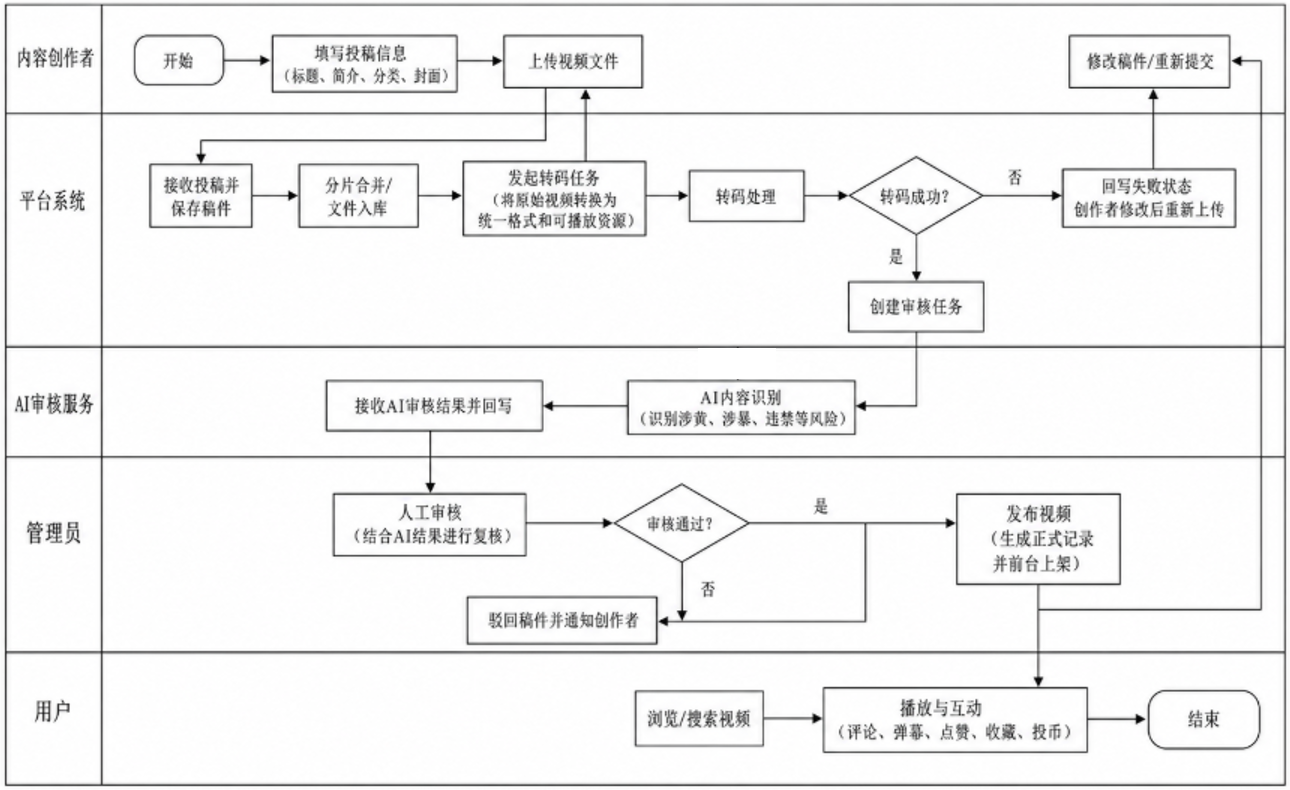
\includegraphics[width=\textwidth]{images/system_business_flow.png}
    \caption{系统总体业务流程图}
    \label{fig:system-business-flow}
\end{figure}

\section{用户端功能需求分析}
\label{sec:user-side-requirements}

用户端功能主要围绕公开视频浏览、视频检索、在线播放、社区互动和账号认证等内容展开，其主要功能需求如表~\ref{tab:user-main-functions} 所示。

\begin{table}[htbp]
  \centering
  \caption{用户端主要功能需求}
  \label{tab:user-main-functions}
  \begin{tabular}{p{0.22\textwidth}p{0.32\textwidth}p{0.36\textwidth}}
    \hline
    \textbf{功能类别} & \textbf{功能点} & \textbf{需求说明} \\
    \hline
    基础浏览 & 首页视频列表、分类筛选 & 用户能够查看公开视频内容 \\
    搜索检索 & 关键词搜索、排序、热词 & 用户能够根据标题、简介、标签查找视频 \\
    视频播放 & 视频详情、分 P 切换、在线播放 & 用户能够稳定播放已发布视频 \\
    用户互动 & 评论、弹幕、点赞、收藏、投币、关注 & 登录用户能够参与社区互动 \\
    账号功能 & 注册、登录、退出、自动登录 & 支持用户身份识别和状态维护 \\
    \hline
  \end{tabular}
\end{table}

\subsection{游客访问与用户认证需求}
\label{subsec:visitor-auth-requirements}

此平台应可允许游客浏览公开视频、查看视频详情和使用搜索功能，以降低用户进入平台的门槛。但涉及用户身份绑定的操作，例如评论、弹幕、点赞、收藏、投币和关注等，应要求用户登录后才能进行。

注册用户需要支持注册、登录、退出和登录状态校验等功能。登录后，系统应能够识别当前用户身份，并根据身份允许其执行互动操作。普通用户登录态与管理员登录态应保持区分，避免后台权限被普通用户误用或越权访问。权限控制通常需要结合认证与授权机制进行设计，Spring Security 文档也对认证和访问控制能力进行了说明\cite{springsecuritydocs}。

\subsection{视频浏览、搜索与播放需求}
\label{subsec:browse-search-play-requirements}

视频浏览是用户端的基础功能。系统需要支持首页视频列表、分类筛选、视频详情展示和分 P 播放等功能。首页和分类页面应展示视频封面、标题、作者、发布时间和基础统计数据，方便用户快速了解视频内容。

搜索功能需要支持用户根据关键词查找视频。检索范围可以包括视频标题、简介和标签等字段，并支持按相关性、发布时间或热度进行排序。对于内容类平台而言，搜索功能能够弥补单纯首页展示的不足，帮助用户主动发现目标内容。Elasticsearch 等全文检索技术可以为复杂关键词检索提供支持\cite{elasticsearchdocs}。

播放功能需要能够稳定加载已发布视频的播放资源。由于上传视频通常需要经过转码和切片处理，播放页应支持加载 HLS 资源，并在播放失败时给出明确提示。HLS 协议通过播放列表和媒体分片组织视频资源，适合网页端在线播放场景\cite{rfc8216hls}。

\subsection{社区互动需求}
\label{subsec:interaction-requirements}

社区互动是视频分享平台区别于普通视频播放工具的重要特点。系统需要支持评论、弹幕、点赞、收藏、投币和关注等功能。评论用于表达用户观点，弹幕与视频播放时间点相关，点赞、收藏、投币和关注用于记录用户对内容或作者的偏好。

对于互动行为，系统需要避免同一用户重复执行不合理操作，例如重复点赞或重复收藏。系统还应在用户再次进入视频详情页时展示当前互动状态，使用户能够清楚看到自己是否已点赞、收藏或关注。

\section{创作中心功能需求分析}
\label{sec:creator-center-requirements}

创作中心主要面向内容创作者，功能需求集中在视频投稿、分片上传、文件处理、稿件状态查看和作品管理等方面，其主要功能需求如表~\ref{tab:creator-functions} 所示。

\begin{table}[htbp]
  \centering
  \caption{创作中心功能需求}
  \label{tab:creator-functions}
  \begin{tabular}{p{0.22\textwidth}p{0.32\textwidth}p{0.36\textwidth}}
    \hline
    \textbf{功能类别} & \textbf{功能点} & \textbf{需求说明} \\
    \hline
    投稿信息 & 标题、分类、标签、简介、封面 & 保存视频基础内容信息 \\
    视频上传 & 分片上传、多文件上传 & 支持大文件稳定上传 \\
    文件处理 & 分片合并、视频转码、播放资源生成 & 使视频满足在线播放要求 \\
    状态查看 & 转码中、待审核、审核通过、审核失败 & 创作者可查看稿件处理进度 \\
    作品管理 & 稿件列表、编辑、删除、统计查看 & 创作者可管理个人投稿内容 \\
    \hline
  \end{tabular}
\end{table}

\subsection{视频投稿需求}
\label{subsec:video-submit-requirements}

创作中心面向内容创作者，主要承担视频投稿和作品管理功能。创作者需要能够填写视频标题、选择分类、上传封面、填写标签和简介，并设置投稿相关选项。投稿功能的目标不是简单上传文件，而是将视频资源、基础信息和后续审核流程关联起来。

视频投稿应支持多分 P 或多文件场景。对于系列视频或较长视频，创作者可能需要上传多个视频片段。系统需要保存每个分 P 的标题、文件信息和排序关系，使用户在播放页可以切换分 P，管理员在审核时也可以分别查看不同文件内容。

\subsection{视频上传与文件处理需求}
\label{subsec:upload-file-processing-requirements}

视频文件通常体积较大，直接一次性上传容易受到网络波动影响。因此，系统需要支持大文件分片上传。前端将文件拆分为多个分片后逐个上传，服务端接收分片并保存临时文件，在所有分片上传完成后进行合并。

上传完成后，系统还需要对视频进行转码处理。不同设备上传的视频格式和编码方式可能不同，若不统一处理，可能导致前台播放兼容性差。FFmpeg 可用于完成视频转码、格式转换和切片等处理\cite{ffmpegdocs}。从用户体验角度看，视频上传、转码和审核不应要求用户长时间等待，系统应通过稿件状态展示处理进度。

\subsection{稿件状态与作品管理需求}
\label{subsec:post-status-work-management}

创作者提交视频后，需要了解稿件当前处于什么阶段，例如转码中、转码失败、待审核、审核通过或审核不通过。状态设计应尽量清晰，避免使用用户难以理解的内部状态名称。

作品管理功能应支持查看稿件列表、查看视频状态、编辑未发布稿件、删除不需要的稿件，以及查看作品基础统计信息。作品管理页面应突出投稿时间、审核结果和处理状态，而不是只展示视频封面和播放量。

\section{管理端与 AI 审核需求分析}
\label{sec:admin-ai-requirements}

管理端与 AI 审核模块主要用于支撑后台认证、分类维护、视频人工审核、AI 审核任务处理和审核结果展示等功能，其主要需求如表~\ref{tab:admin-ai-functions} 所示。

\begin{table}[htbp]
  \centering
  \caption{管理端与 AI 审核功能需求}
  \label{tab:admin-ai-functions}
  \begin{tabular}{p{0.24\textwidth}p{0.32\textwidth}p{0.34\textwidth}}
    \hline
    \textbf{功能类别} & \textbf{功能点} & \textbf{需求说明} \\
    \hline
    管理员认证 & 后台登录、退出、权限校验 & 保证后台功能只对管理员开放 \\
    分类管理 & 分类新增、编辑、删除、排序 & 维护平台内容分类体系 \\
    视频审核 & 审核列表、审核详情、通过、驳回 & 控制视频是否正式发布 \\
    AI 审核任务 & 自动创建任务、投递请求、接收结果 & 辅助完成视频内容风险识别 \\
    AI 结果展示 & 风险等级、风险标签、命中片段、原因说明 & 帮助管理员快速定位风险内容 \\
    \hline
  \end{tabular}
\end{table}

\subsection{管理员认证与分类管理需求}
\label{subsec:admin-category-requirements}

管理端主要面向平台管理员。管理员需要通过后台登录后才能进入管理系统，普通用户不能直接访问后台接口。后台接口应进行身份校验，未登录或权限不足时应拒绝访问。

分类管理是后台管理中的基础功能。视频分类会影响用户投稿时的分类选择，也会影响前台视频展示、筛选和搜索。因此，系统需要支持管理员维护视频分类数据，包括新增分类、修改分类、删除分类、排序和启用停用等操作。

\subsection{人工审核与 AI 审核需求}
\label{subsec:manual-ai-audit-requirements}

视频人工审核是管理端的核心需求。创作者提交视频后，视频不能直接进入正式发布状态，而需要经过转码和审核流程。管理员需要能够查看待审核视频列表，进入审核详情页，观看视频内容，查看投稿信息和 AI 审核结果，并做出通过或驳回决定。

AI 审核服务主要负责自动化风险识别。系统在视频转码完成后应创建 AI 审核任务，并将待审核视频信息发送给 AI 服务。AI 服务完成分析后，应返回审核建议、风险等级、风险标签、命中片段和原因说明等信息。AI 审核结果不直接决定视频最终发布，而是为管理员人工审核提供辅助依据。人机交互研究中也指出，AI 系统应为人工决策提供可理解、可纠错的支持，而不是完全替代人工判断\cite{amershi2019guidelines}。

\subsection{视频状态流转需求}
\label{subsec:video-status-flow-requirements}

为了保证审核流程清晰，系统中视频状态需要明确流转。投稿视频从用户提交开始，通常会经历转码中、转码失败、待审核、审核通过或审核不通过等状态。视频状态流转如图~\ref{fig:video-status-flow} 所示。

\begin{figure}[htbp]
  \centering
  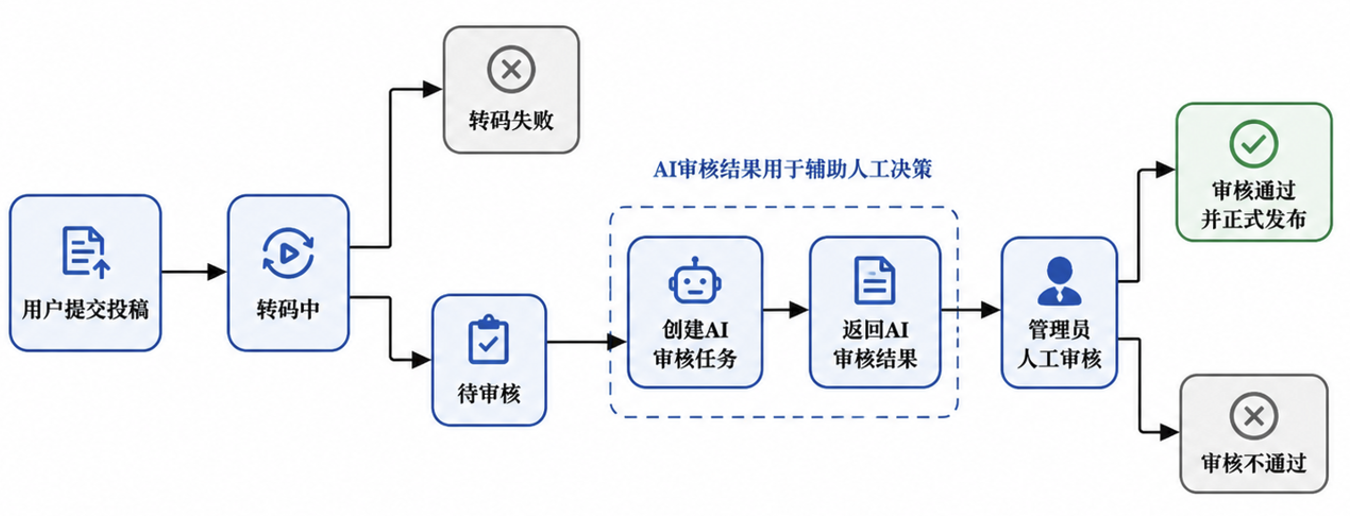
\includegraphics[width=0.95\textwidth]{images/video-status-flow.png}
  \caption{视频投稿与审核状态流转图}
  \label{fig:video-status-flow}
\end{figure}

由图~\ref{fig:video-status-flow} 可知，视频是否能够发布并不只取决于用户是否提交投稿，还取决于视频是否转码成功以及管理员是否审核通过。该状态流转规则为后续总体设计和详细实现提供了需求依据。

\section{非功能需求分析}
\label{sec:non-functional-requirements}

非功能需求主要关注系统质量属性。本系统需要在性能、可扩展性、安全性、可靠性、一致性和可维护性方面满足基本要求。

性能方面，登录、视频列表、视频详情、评论加载和搜索查询等常规接口应保持较好的响应速度；视频上传、视频转码和 AI 审核等耗时任务应采用异步处理方式，避免用户长时间等待。ISO/IEC 25010 软件质量模型将性能效率作为软件质量的重要方面\cite{iso25010}。

可扩展性方面，系统应支持后续根据业务压力扩展不同模块，例如资源处理压力较大时可以优先优化资源服务，互动访问频繁时可以优化互动模块。安全性方面，系统需要区分普通用户和管理员权限，对后台接口、上传文件和审核接口进行必要保护。

可靠性和一致性方面，系统应保证视频投稿、文件处理、审核状态和正式发布数据之间保持逻辑一致。对于涉及多个服务协作的关键写操作，系统需要具备事务协调或状态补偿能力；对于视频转码、AI 审核和播放统计等耗时或高频任务，则应通过异步处理和结果回写保证最终状态一致。若转码失败、AI 审核失败或服务短暂不可用，系统应能记录状态和失败原因，避免业务状态混乱。可维护性方面，系统应保持清晰的模块边界、接口规范和日志记录，便于后续修改和排查问题。

系统主要非功能需求如表~\ref{tab:non-functional-requirements} 所示。

\begin{table}[htbp]
  \centering
  \caption{系统主要非功能需求}
  \label{tab:non-functional-requirements}
  \begin{tabular}{p{0.20\textwidth}p{0.36\textwidth}p{0.34\textwidth}}
    \hline
    \textbf{非功能需求} & \textbf{需求说明} & \textbf{设计关注点} \\
    \hline
    性能需求 & 常规页面和接口响应应保持流畅 & 缓存、搜索、异步任务处理 \\
    可扩展性 & 系统应便于后续增加功能和扩展服务 & 模块拆分、服务边界、接口规范 \\
    安全性 & 区分普通用户和管理员权限，保护内部接口 & 身份认证、权限校验、上传限制 \\
    可靠性 & 异常情况下核心流程应尽量不中断 & 状态记录、失败原因、人工处理 \\
    数据一致性 & 投稿、转码、审核和发布状态应保持一致 & 事务控制、状态流转、结果回写 \\
    可维护性 & 系统结构清晰，便于后续修改和扩展 & 分层设计、公共模块、日志和文档 \\
    \hline
  \end{tabular}
\end{table}